\chapter{Diseño de la Solución} \label{sec:Metodos}

% ── Paleta de colores para diagramas MCDA ────────────────────────────────────
\definecolor{oe3azul}    {HTML}{1A3F6F}   % encabezados principales
\definecolor{oe3azulcl}  {HTML}{E8EEF7}   % filas alternas
\definecolor{oe3verde}   {HTML}{1B5E20}   % Excelente
\definecolor{oe3verdecl} {HTML}{E8F5E9}
\definecolor{oe3ambar}   {HTML}{E65100}   % Aceptable
\definecolor{oe3ambarcl} {HTML}{FFF3E0}
\definecolor{oe3rojo}    {HTML}{B71C1C}   % Deficiente
\definecolor{oe3rojocl}  {HTML}{FFEBEE}
\definecolor{oe3gris}    {HTML}{546E7A}   % subtítulos
\definecolor{oe3griscl}  {HTML}{F5F5F5}  % fondo de notas

A partir de la planificación Scrum (\cref{cap:metodologia}), este capítulo presenta el diseño de la solución telemática. El diseño responde directamente a las causas del árbol de problemas y se estructura en cuatro pilares: una arquitectura de red controlada, un sistema de medición de Calidad de Servicio (QoS), un modelo de decisión multicriterio (MCDA) y una estrategia de seguridad automatizada bajo el principio de Zero Trust. El detalle de implementación y despliegue de cada componente se documenta en el \cref{cap:herramienta}.


El diseño responde directamente a las causas identificadas en el árbol de problemas: la ausencia de criterios objetivos para seleccionar el componente de red (CNI), la falta de visibilidad sobre el tráfico interno del clúster y el sobredimensionamiento de recursos que resulta de operar sin datos reales \cite{ref29}. La solución se estructura en cuatro pilares: una arquitectura de red controlada, un sistema de medición de Calidad de Servicio (QoS), un modelo de decisión multicriterio (MCDA) y una estrategia de seguridad automatizada.

\section{Arquitectura de Red y Topología}

El entorno de pruebas se diseñó para que el CNI sea la única variable entre ciclos de medición; el hardware, el sistema operativo, la topología y la duración de las pruebas permanecen constantes en todos los escenarios.

\subsection{Red underlay}

La red underlay constituye la infraestructura física sobre la que opera el clúster. Se optó por la nube pública de DigitalOcean en lugar de servidores físicos propios, ya que la homogeneidad del entorno elimina el ruido de hardware local ---variabilidad de NIC, temperatura, interferencias--- y garantiza que cualquier diferencia medida en throughput, latencia o CPU sea atribuible al CNI y no al sustrato. El aprovisionamiento se realizó mediante Terraform, herramienta de Infraestructura como Código (IaC): la configuración completa de los servidores queda descrita en archivos versionados, lo que permite reproducir el entorno de forma idéntica. Esta reproducibilidad es una condición necesaria para la validez del experimento, pues sin ella la comparación entre CNIs pierde valor probatorio \cite{ref7}.

Se utilizó K3s ---distribución liviana de Kubernetes--- con un nodo Master, datastore PostgreSQL gestionado por DigitalOcean y dos nodos Worker dedicados. El menor \emph{footprint} de K3s frente a Kubernetes estándar deja una mayor proporción de CPU y RAM disponible para el CNI, lo que aumenta la sensibilidad de las mediciones; el datastore externo elimina el punto único de fallo del plano de control sin la complejidad operativa de un clúster etcd. La topología incluye una red privada VPC para el tráfico interno entre nodos, de manera que la latencia medida dependa exclusivamente de la eficiencia del CNI y no de la variabilidad de Internet público \cite{ref8}.

\subsection{Red overlay y CNI evaluados}

La red overlay, implementada por el plugin CNI, provee la conectividad entre cargas de trabajo distribuidas en distintos nodos. Kubernetes no incluye esta funcionalidad por defecto y delega la elección del CNI en cada organización \cite{ref4,ref18}; esa libertad de elección, ejercida sin criterios objetivos basados en mediciones, es el problema central que aborda este trabajo.

El núcleo del diseño es la comparativa de cuatro CNI con filosofías de implementación distintas (Tabla~\ref{tab:cni-evaluados}).

\begin{table}[htbp]
\centering
\scriptsize
\caption{CNI evaluados: tecnología base, versión desplegada y enfoque.}
\label{tab:cni-evaluados}
\begin{tabularx}{\textwidth}{|Y|Y|Y|Y|}
\hline
\textbf{CNI} & \textbf{Tecnología Base} & \textbf{Versión} & \textbf{Enfoque} \\
\hline
Flannel & VXLAN (L2) & nativo K3s & Overlay sencillo de instalar; sin soporte nativo de NetworkPolicies. \\
\hline
Calico & VXLAN (DO VPC) & 3.29.1 Tigera Operator & Tigera Operator con \texttt{encapsulation: VXLAN}; políticas avanzadas L3/L4. \\
\hline
Cilium & eBPF + VXLAN tunnel & 1.16.5 & \texttt{routingMode=tunnel}, \texttt{tunnelProtocol=vxlan}; opera en el kernel con eBPF y filtrado L7 HTTP nativo. \\
\hline
Antrea & OVS (SDN) & 2.2.0 & Open vSwitch con sistema jerárquico de Tiers (Emergency $>$ SecurityOps $>$ NetworkOps $>$ Platform $>$ Application). \\
\hline
\end{tabularx}
\end{table}

Las tecnologías base de estos CNI sustentan dataplanes diferentes. \textbf{VXLAN} crea redes virtuales sobre redes físicas existentes encapsulando los paquetes originales dentro de paquetes UDP, lo que permite transportar tráfico de capa 2~\cite{ref19} sobre redes de capa 3; el costo es un \emph{overhead} de 50 bytes por paquete, que puede reducir el throughput efectivo en transferencias de paquetes pequeños \cite{ref12}. \textbf{eBPF} permite ejecutar programas de forma segura dentro del kernel de Linux; aplicado a redes, posibilita que Cilium intercepte y redirija paquetes sin copiarlos al espacio de usuario, eliminando una fuente principal de latencia \cite{ref27}. \textbf{Open vSwitch (OVS)} es un switch virtual orientado a SDN \cite{ref22} que Antrea emplea para implementar conectividad y políticas mediante un sistema de Tiers jerárquico, capaz de expresar reglas corporativas con mayor prioridad que las NetworkPolicies estándar de Kubernetes.

La selección de estos cuatro CNI no es arbitraria: cada uno aporta un punto de comparación específico y un riesgo característico a medir. Flannel actúa como línea base de conectividad sencilla, con el riesgo de carecer de \emph{enforcement} nativo de NetworkPolicies. Calico aporta madurez operativa y políticas de red en producción, con un posible costo por la evaluación de reglas. Cilium representa el uso de eBPF como mecanismo moderno de aceleración, visibilidad y políticas L7, a cambio de mayor complejidad conceptual y mayor consumo de RAM. Antrea aporta una aproximación basada en OVS y conceptos de SDN, con dependencia de componentes adicionales. En conjunto, cubren el espectro de opciones que enfrenta un equipo de operaciones real, desde la simplicidad operativa hasta las capacidades avanzadas de observabilidad y seguridad.

\section{Sistema de Medición de Calidad de Servicio (QoS)}

La Calidad de Servicio (QoS) cuantifica el comportamiento real de la red desde la perspectiva de las aplicaciones. El sistema de medición sigue los principios de la metrología de redes ---control de variables, reproducibilidad y representatividad estadística--- para que las diferencias observadas sean atribuibles al CNI y no al procedimiento de medición.

\subsection{Inyección de tráfico}

El tráfico se genera con iperf3, herramienta de referencia para pruebas de rendimiento de redes, que opera con un modelo cliente-servidor en el que un Pod emisor envía tráfico a un Pod receptor y ambos registran estadísticas detalladas de la transferencia. Para asegurar tráfico inter-nodo, el cliente y el servidor se separan mediante \texttt{podAntiAffinity} suave (\texttt{preferredDuringSchedulingIgnoredDuringExecution}, weight~100): con dos Workers disponibles, el scheduler los ubica en nodos distintos en la práctica, y la modalidad \texttt{preferred} ---en lugar de \texttt{required}--- mantiene la resiliencia ante reinicios de nodo. La ejecución se automatiza mediante CronJobs de Kubernetes, con ráfagas de tráfico TCP de 300 segundos cada 30 minutos, frecuencia que captura el comportamiento de la red en distintos momentos y compone un perfil estadístico representativo \cite{ref7}.

\subsection{Variables telemáticas capturadas}

El sistema de medición parte del principio de que una métrica aislada no describe la calidad de una red. La Tabla~\ref{tab:variables-qos} resume las variables capturadas, que combinan rendimiento de red, estabilidad y costo computacional; la latencia se registra en sus valores mínimo, promedio, máximo y de variabilidad (\emph{jitter}), de modo que los picos no queden ocultos por el promedio.

\begin{table}[htbp]
\centering
\scriptsize
\caption{Variables telemáticas capturadas por el sistema de medición.}
\label{tab:variables-qos}
\begin{tabularx}{\textwidth}{|Y|Y|Y|}
\hline
\textbf{Variable QoS} & \textbf{Unidad de medida} & \textbf{Relevancia} \\
\hline
Throughput (ancho de banda efectivo) & Gbps / Mbps & Capacidad efectiva de transferencia entre Pods. Herramienta: iperf3 \texttt{-J}, 300 s TCP. \\
\hline
Latencia de establecimiento TCP & ms (min/avg/max/mdev) & Costo de iniciar una comunicación entre servicios. Herramienta: script Bash con \texttt{nc -z -w 2}, 30 muestras por corrida. \\
\hline
Retransmisiones TCP & número de paquetes & Indicador de inestabilidad en el canal de encapsulamiento del CNI. \\
\hline
Costo computacional del CNI & \% CPU / MB RAM & Recursos que consume el propio CNI para procesar el tráfico; determina el impacto en el sobredimensionamiento. \\
\hline
\end{tabularx}
\end{table}

\subsection{Pila de observabilidad: Prometheus y Grafana}

\textbf{Prometheus} recolecta métricas mediante un modelo de \emph{scraping} periódico sobre cada nodo, registrando estadísticas de CPU, memoria, red y estado del CNI. El almacenamiento en series temporales permite correlacionar el consumo de recursos del agente CNI con los instantes exactos de las pruebas de throughput, verificando que las métricas de eficiencia reflejen el comportamiento bajo carga y no en reposo \cite{ref6}. \textbf{Grafana} constituye la capa de visualización: presenta en dashboards interactivos el throughput, la latencia, el consumo de CPU del agente y las retransmisiones TCP. Esta visibilidad permitió detectar anomalías durante las sesiones ---picos de CPU o reinicios inesperados del agente--- antes de que comprometieran la integridad de las corridas \cite{ref6}.

\section{Modelo de Decisión Multicriterio (MCDA)} \label{sec:apb_intro}

Para resolver la selección objetiva del CNI se diseñó un modelo de Análisis de Decisión Multicriterio (MCDA), enfoque empleado en ingeniería y economía cuando una decisión involucra múltiples factores con distinta importancia \cite{ref34}. A diferencia de una comparación basada en un único criterio ---por ejemplo, el throughput máximo---, el MCDA captura el \emph{trade-off} entre velocidad, eficiencia de recursos y capacidades de seguridad, y produce una recomendación que refleja las prioridades de cada tipo de organización.

El reto principal de elegir un CNI es que no existe una única solución óptima en todas las dimensiones simultáneamente. El rendimiento base de velocidad de red (\emph{throughput}) es solo una dimensión del problema. Por ejemplo, una pasarela de transacciones bancarias exige seguridad estricta y aislamiento lógico, mientras que un clúster IoT en nodos con recursos de cómputo limitados prioriza un bajo consumo de memoria RAM y CPU. La Tabla~\ref{tab:apb_tradeoffs} muestra a nivel conceptual este compromiso de rendimiento (\emph{trade-off}) cualitativo entre los plugins evaluados, sirviendo de introducción visual al dilema de selección.

\begin{table}[htbp]
\centering
\scriptsize
\caption{Matriz comparativa cualitativa de compromisos (trade-offs) en CNIs.}
\label{tab:apb_tradeoffs}
\begin{tabularx}{\textwidth}{|Y|c|c|c|c|}
\hline
\textbf{Dimensión} & \textbf{Flannel} & \textbf{Calico} & \textbf{Cilium} & \textbf{Antrea} \\
\hline
Latencia y jitter & Medio & Excelente & Bueno & Aceptable \\
Throughput & Bueno & Excelente & Aceptable & Bueno \\
Consumo de CPU & Excelente & Deficiente & Aceptable & Aceptable \\
Consumo de RAM & Excelente & Deficiente & Aceptable & Aceptable \\
Network Policies L4 & Nulo (No soporta) & Excelente & Excelente & Excelente \\
Network Policies L7 & Nulo (No soporta) & Nulo (No soporta) & Excelente & Nulo (No soporta) \\
\hline
\end{tabularx}
\end{table}

\subsection{Definición de criterios y métricas de evaluación} \label{sec:apb_criterios}

Para comparar los plugins de manera objetiva, el modelo agrupa los indicadores en tres criterios principales (C1, C2 y C3), resumidos en la Tabla~\ref{tab:apb_criterios}.

\begin{table}[htbp]
\centering
\scriptsize
\caption{Estructura de criterios, preguntas de control y métricas del modelo de selección.}
\label{tab:apb_criterios}
\begin{tabularx}{\textwidth}{|l|l|Y|}
\hline
\textbf{Criterio Principal} & \textbf{Pregunta de Control (UI)} & \textbf{Métricas y Variables Asociadas} \\
\hline
\textbf{C1: Rendimiento de Red (QoS)} & ¿Qué tan rápido tiene que responder? & Latencia base promedio (ms), Latencia máxima (ms) \\
\cline{2-3}
& ¿Qué tan estable debe ser la conexión? & Jitter (MDEV) (ms), Retransmisiones TCP (paquetes/sesión) \\
\cline{2-3}
& ¿Cuántos datos se van a mover al mismo tiempo? & Throughput TCP promedio (Mbps) \\
\hline
\textbf{C2: Eficiencia de Recursos} & ¿Los servidores donde va a funcionar son pequeños? & Consumo de CPU promedio (\% del nodo), Consumo de RAM promedio (MB) \\
\hline
\textbf{C3: Impacto de Seguridad} & ¿Qué tan importante es la seguridad y el control? & Soporte nativo de Network Policies, Sobrecarga (overhead) de latencia y throughput (\%) \\
\hline
\end{tabularx}
\end{table}

\begin{itemize}
  \item \textbf{C1 --- Rendimiento de red (QoS):} Evalúa latencia promedio/máxima, inestabilidad (\emph{jitter}), velocidad de transferencia (\emph{throughput}) y retransmisiones (pérdida de paquetes).
  \item \textbf{C2 --- Eficiencia de recursos:} Mide el consumo de CPU y memoria RAM que el agente CNI requiere en cada nodo worker para funcionar.
  \item \textbf{C3 --- Impacto de seguridad:} Mide la sobrecarga (\emph{overhead}) de latencia y throughput al activar Network Policies en el clúster.
\end{itemize}

\subsection{Limpieza estadística con el Rango Intercuartílico (IQR)}

Antes de aplicar el modelo, los datos recolectados pasan por una limpieza estadística mediante el Rango Intercuartílico (IQR), que elimina \emph{outliers} causados por eventos externos como mantenimientos del proveedor o picos de uso compartido. El criterio de corte emplea las \emph{vallas} de Tukey ($Q_1 - 1{,}5\cdot\text{IQR}$, $Q_3 + 1{,}5\cdot\text{IQR}$), regla clásica del análisis exploratorio de datos para identificar valores atípicos~\cite{ref32}. Este procesamiento evita que la recomendación dependa de valores atípicos o de la magnitud numérica de una métrica, y se implementa en el script \texttt{docs/procesador.js}.

\subsection{Normalización continua Min-Max} \label{sec:apb_umbrales}

Para estandarizar las métricas crudas y permitir la suma ponderada del modelo MCDA, el algoritmo procesador aplica una función de normalización \emph{min-max} continua que proyecta los valores a una escala uniforme de $1.00$ a $5.00$. A diferencia de los modelos basados en umbrales discretos escalonados, esta aproximación refleja proporcional y exactamente las brechas de rendimiento entre los plugins evaluados.

La transformación de las métricas empíricas se realiza mediante el método de escalamiento lineal Min-Max, de acuerdo con la formulación analizada por \cite{ref35} y revisada en los surveys de técnicas de normalización en MCDA~\cite{ref36}. La Ecuación~\eqref{eq:mcda-norm} define la transformación directa para las métricas donde un mayor valor representa un mejor desempeño (ej. \emph{throughput}), mientras que la Ecuación~\eqref{eq:apb_minmax_inv} describe la transformación para aquellas dimensiones donde un menor valor es deseable (ej. latencia, retransmisiones, consumo de CPU y RAM).

\begin{equation}
  V_{norm} = 1 + \left( \frac{V_{crudo} - Min}{Max - Min} \right) \times 4
  \label{eq:mcda-norm}
\end{equation}

\begin{equation}
  V_{norm} = 1 + \left( \frac{Max - V_{crudo}}{Max - Min} \right) \times 4
  \label{eq:apb_minmax_inv}
\end{equation}

Los resultados normalizados garantizan que el CNI con el mejor desempeño en una dimensión obtenga exactamente $5.00$ y el de peor desempeño obtenga exactamente $1.00$.

\subsection{Factores de ponderación y restricciones no compensatorias} \label{sec:apb_ponderaciones}

El modelo aplica factores de ponderación (pesos porcentuales) que suman el $100\%$ ($1,0$), asignando mayor peso a las métricas más críticas según el caso de uso. La distribución de pesos calculados dinámicamente por la herramienta para los tres perfiles base se muestra en la Tabla~\ref{tab:apb_pesos}.

\begin{table}[htbp]
\centering
\scriptsize
\caption{Matriz de factores de ponderación (pesos calculados) por perfil de la tesis.}
\label{tab:apb_pesos}
\begin{tabularx}{\textwidth}{|Y|c|c|c|c|c|}
\hline
\textbf{Perfil / Caso de Uso} & \textbf{Latencia} & \textbf{Estabilidad} & \textbf{Throughput} & \textbf{Recursos} & \textbf{Seguridad} \\
\hline
Fintech / Seguridad crítica & 20.8\% & 24.8\% & 21.0\% & 8.1\% & 25.3\% \\
\hline
Streaming / Alto rendimiento & 27.7\% & 22.7\% & 25.1\% & 12.3\% & 12.3\% \\
\hline
IoT / Recursos limitados & 20.8\% & 19.0\% & 18.5\% & 28.0\% & 13.7\% \\
\hline
\end{tabularx}
\end{table}

\subsubsection{Restricción no compensatoria de seguridad}

Para evitar que un CNI inseguro gane por pura eficiencia computacional, el modelo combina el método compensatorio SAW con una restricción conjuntiva, siguiendo los modelos no compensatorios de decisión multiatributo~\cite{ref31}. Si el perfil exige un nivel de seguridad \emph{Alto} o \emph{Muy Alto} (valor $\ge 4$ en el recomendador, como ocurre en el perfil Fintech), cualquier CNI que carezca de soporte nativo para Network Policies (como Flannel) sufre una penalización. Esto reduce su puntaje general al $40\%$ del valor ponderado calculado:

\begin{equation}
  P_{\text{final}} =
  \begin{cases}
    P_{\text{MCDA}} \times 0,40 & \text{si la seguridad es prioritaria y el CNI carece de políticas} \\
    P_{\text{MCDA}}               & \text{en caso normal}
  \end{cases}
  \label{eq:mcda-penalizacion}
\end{equation}

Esta restricción matemática asegura que los plugins con falencias críticas en el plano de seguridad sean descartados automáticamente en entornos regulados, invalidando victorias engañosas logradas puramente mediante ventajas en la eficiencia de recursos computacionales. El factor $\alpha = 0.40$ (reducción del 60\,\%) es un umbral de diseño calibrado para que la penalización sea severa sin anular por completo el puntaje, lo que permite que el recomendador conserve el ordenamiento relativo del resto de dimensiones para fines de diagnóstico.

\subsection{Modelo matemático de decisión multicriterio (MCDA)} \label{sec:apb_mcda}

Para la recomendación formal del CNI, el algoritmo aplica el modelo MCDA de sumatoria ponderada clásica o SAW (Simple Additive Weighting), fundamentado en la teoría clásica de decisiones multicriterio~\cite{ref34,ref37}:

\begin{equation}
  P_{\text{CNI}} = \sum_{i=1}^{n} V_i \times W_i
  \label{eq:mcda-suma}
\end{equation}

Donde $P_{\text{CNI}}$ es el puntaje del plugin para el perfil; $V_i$ es la puntuación normalizada asignada según la métrica $i$; $W_i$ es el peso porcentual de la métrica en el perfil; y $n$ es el número de métricas evaluadas. 

La escala final de los puntajes del modelo MCDA está normalizada en la escala de $1,0$ a $5,0$, donde una puntuación de $5,0$ representa un CNI con comportamiento ideal (cumplimiento excelente de todos los requisitos prioritarios) y $1,0$ representa un cumplimiento totalmente deficiente del perfil evaluado.

El flujo de procesamiento del recomendador interactivo se resume a continuación:

\begin{center}
  \begin{tabular}{ccccccc}
    \colorbox{oe3azulcl}{\small\textbf{JSON/CSV crudos}} &
    $\rightarrow$ &
    \colorbox{oe3griscl}{\small\textbf{Filtro IQR}} &
    $\rightarrow$ &
    \colorbox{oe3griscl}{\small\textbf{Norm.\ min-max}} &
    $\rightarrow$ &
    \colorbox{oe3verdecl}{\small\textbf{$\sum V_i \times W_i$}} \\[6pt]
    \multicolumn{7}{c}{$\downarrow$} \\[4pt]
    \multicolumn{7}{c}{\colorbox{oe3azulcl}{\small\textbf{$P_{\text{CNI}}$: El CNI con la puntuación más alta es la recomendación del modelo}}}
  \end{tabular}
\end{center}


\section{Seguridad y Micro-segmentación (Zero Trust)}

En su configuración inicial, cualquier aplicación dentro del clúster puede comunicarse con cualquier otra. Las Network Policies permiten implementar el principio de \emph{Zero Trust}: conceder solo lo necesario y verificar explícitamente cada acceso \cite{ref24,ref25}. Esto reduce la superficie de ataque, ya que ante el compromiso de un Pod las políticas limitan el movimiento lateral a las rutas explícitamente autorizadas. La aplicación efectiva de estas políticas depende del CNI: si el plugin no las implementa en su plano de datos, la política existe como objeto declarativo sin producir efecto \cite{ref4,ref18}.

\subsection{Alcance operativo declarado} \label{sec:apb2_alcance}

El enunciado original del OE2 introduce dos términos ---\emph{superficie de ataque} y \emph{probabilidad de incidentes de seguridad}--- que pertenecen al vocabulario de la gestión de riesgos pero que no fueron medidos en este trabajo con métricas cuantitativas estándar de la industria (recuento de CVE, técnicas MITRE ATT\&CK bloqueadas, modelos formales de amenazas). Para sostener la evaluación con la evidencia disponible, se establecen las siguientes definiciones operativas, que se aplican a lo largo del manuscrito.

\begin{itemize}
    \item \textbf{Superficie de ataque} se define operativamente como el \emph{conjunto de flujos de red autorizados entre Pods o namespaces del clúster}. Su reducción se observa cuando el número de pares (origen, destino, puerto) permitidos por la política declarativa disminuye respecto al estado por defecto del clúster, donde toda comunicación interna está permitida. El bloqueo efectivo de un flujo no autorizado en una prueba de conectividad ---por ejemplo, el rechazo del tráfico Frontend$\rightarrow$Database en TC-SEC-04--- constituye evidencia directa de esta reducción.

    \item \textbf{Probabilidad de incidentes de seguridad} se define como una \emph{aproximación cualitativa} de la capacidad del CNI para bloquear los movimientos laterales y los egresos prohibidos declarativamente en los tres casos de uso ejecutados (\texttt{zero\_trust}, \texttt{multi\_tier} y \texttt{egress\_block}). No se trata de una probabilidad estadística calculada a partir de una frecuencia base de incidentes; es una proxy observacional que permite comparar capacidades de \emph{enforcement} entre CNIs.

    \item \textbf{Vulnerabilidades a reducir} se entienden como \emph{configuraciones inseguras por defecto} ---comunicación inter-Pod abierta, ausencia de \emph{default-deny}, egress externo no controlado, ausencia de segmentación entre tiers de aplicación---, no como CVE conocidos en el código del CNI o de Kubernetes.
\end{itemize}

Esta delimitación es requerida para evaluar la \emph{configuración} de políticas de red, no la resistencia del clúster frente a herramientas ofensivas concretas. La distinción se retoma con mayor detalle en la \S\ref{sec:delimitacion_oe2} de la Discusión.

\subsection{Requisitos verificables derivados del OE2} \label{sec:apb2_verbos}

El enunciado del OE2 se descompone en cuatro requisitos verificables (R1--R4), que imponen obligaciones contrastables con evidencia, y dos efectos esperados (E1--E2), cuya validez se sostiene a partir de los resultados de esos requisitos. La Tabla~\ref{tab:apb2_verbos} resume la descomposición y señala, para cada elemento, la sección del manuscrito que aporta la evidencia correspondiente.

\begin{table}[htbp]
\centering
\scriptsize
\caption{Descomposición del OE2 en requisitos verificables y efectos esperados.}
\label{tab:apb2_verbos}
\begin{tabularx}{\textwidth}{|c|l|Y|Y|}
\hline
\textbf{Id} & \textbf{Requisito} & \textbf{Obligación a demostrar} & \textbf{Anclaje en el manuscrito} \\
\hline
R1 & Configurar de forma segura y automatizada & Políticas de red declarativas, versionadas y aplicadas sin intervención manual sobre el clúster. & \S\ref{sec:apb2_adaptacion} y TC-SEC-08 (\S\ref{sec:apb2_matriz}). \\
\hline
R2 & Adaptar las políticas a cada plugin CNI & Uso de capacidades específicas del CNI, no solo \texttt{NetworkPolicy} estándar de Kubernetes. & \S\ref{sec:apb2_adaptacion}, fragmentos de configuración por CNI. \\
\hline
R3 & Evaluar la reducción de la superficie de ataque & Procedimiento que compare el antes y el después, con y sin políticas, y entre CNIs. & \S\ref{sec:apb2_matriz} y \S\ref{sec:apb2_overhead}. \\
\hline
R4 & Determinar la capacidad de reducir vulnerabilidades & Conclusión técnica trazable a partir de la evidencia de R3. & \S\ref{sec:apb2_mapeo} y Tabla~\ref{tab:cumplimiento-objetivos}. \\
\hline
E1 & Reducir la superficie de ataque & Efecto medible operativamente según \S\ref{sec:apb2_alcance}. & Evidencia: TC-SEC-04, TC-SEC-06, TC-SEC-07. \\
\hline
E2 & Prevenir incidentes de seguridad & Efecto medible operativamente según \S\ref{sec:apb2_alcance}. & Evidencia: \texttt{zero\_trust}, \texttt{multi\_tier}, \texttt{egress\_block}. \\
\hline
\end{tabularx}
\end{table}

\subsection{Matriz extendida de casos de prueba TC-SEC} \label{sec:apb2_matriz}

La Tabla~\ref{tab:apb2_matriz_ext} reescribe la matriz TC-SEC del cuerpo principal (Tabla~\ref{tab:matriz-seguridad}) añadiendo, para cada caso, la amenaza modelada y el requisito del OE2 al que aporta evidencia. Con ello, cada afirmación del objetivo queda trazada hasta la prueba concreta que la respalda y hasta el criterio operativo con el que se verificó.

\begin{table}[htbp]
\centering
\scriptsize
\caption{Matriz extendida TC-SEC: cada caso de prueba, amenaza modelada y requisito del OE2 al que aporta evidencia.}
\label{tab:apb2_matriz_ext}
\begin{tabularx}{\textwidth}{|l|Y|Y|c|}
\hline
\textbf{TC-SEC} & \textbf{Amenaza modelada} & \textbf{Verificación operativa} & \textbf{Requisito} \\
\hline
01 Default Deny Ingress & Comunicación entrante no autorizada hacia el namespace. & \texttt{nc -zv <pod-ip> 8080}; éxito = timeout en \(<5\) s. & R3, E1 \\
\hline
02 Default Deny Egress & Conexiones salientes no autorizadas desde Pods de producción. & \texttt{curl --max-time 3}; éxito = timeout. & R3, E1 \\
\hline
03 Frontend$\rightarrow$Backend permitido & Funcionalidad legítima preservada bajo política activa. & \texttt{nc -zv backend 8080}; éxito = \emph{Connection succeeded}. & R3 \\
\hline
04 Bloqueo Frontend$\rightarrow$Database & Movimiento lateral directo desde la capa de presentación a la capa de datos. & \texttt{nc -zv database 5432}; éxito = \emph{Connection refused} o timeout. & R3, E1, E2 \\
\hline
05 Backend$\rightarrow$Database permitido & Funcionalidad legítima preservada bajo política activa. & \texttt{nc -zv database 5432}; éxito = \emph{Connection succeeded}. & R3 \\
\hline
06 Database no inicia conexiones salientes & Exfiltración o comportamiento anómalo desde la capa de datos. & Egress denegado por política; éxito = bloqueo confirmado. & R3, E2 \\
\hline
07 Bloqueo entre namespaces & Movimiento lateral cruzando límites de namespace. & Pod de \texttt{staging} no alcanza Pods de \texttt{production}; éxito = bloqueo confirmado. & R3, E1, E2 \\
\hline
08 Auto-restauración ArgoCD & Persistencia del estado seguro frente a desviaciones operativas. & Borrado manual; éxito = restauración automática en \(<2\) min. & R1 \\
\hline
\end{tabularx}
\end{table}

La columna ``Requisito'' funciona como traza directa entre cada prueba y el enunciado del OE2. Así, el efecto de \emph{prevenir incidentes} (E2) se respalda en los casos etiquetados con E2 ---TC-SEC-04, 06 y 07---, mientras que la \emph{reducción de la superficie de ataque} (E1) se apoya en TC-SEC-01, 02, 04 y 07; el resto de requisitos se lee de forma análoga.

\subsection{Estrategia de Default Deny}

El diseño implementa Zero Trust en dos niveles: primero, una política de \emph{Default Deny} que bloquea todo el tráfico entrante y saliente de cada namespace; después, una habilitación selectiva que abre únicamente las comunicaciones necesarias. Sobre esta base se definieron tres casos de uso (Tabla~\ref{tab:casos-seguridad}), ejecutados sobre cada CNI que soporta Network Policies ---Calico, Cilium y Antrea---; Flannel se incluye como referencia negativa para confirmar la ausencia de \emph{enforcement} en su plano de datos.

\begin{table}[htbp]
\centering
\scriptsize
\caption{Casos de uso de seguridad implementados por CNI.}
\label{tab:casos-seguridad}
\begin{tabularx}{\textwidth}{|Y|Y|}
\hline
\textbf{Caso} & \textbf{Descripción} \\
\hline
\texttt{zero\_trust} & Default Deny: bloquea todo ingress y egress por defecto; permite solo el tráfico benchmark explícito. \\
\hline
\texttt{multi\_tier} & Reglas explícitas \texttt{frontend $\rightarrow$ backend $\rightarrow$ database} mediante label selectors. Cilium agrega CiliumNetworkPolicy L7 HTTP (solo GET/HEAD desde frontend). \\
\hline
\texttt{egress\_block} & Bloqueo de egress externo con DNS permitido; tráfico inter-pod interno habilitado. \\
\hline
\end{tabularx}
\end{table}

Dos CNI aportan diferenciadores propios. Cilium implementa filtrado HTTP nativo por método mediante \texttt{CiliumNetworkPolicy} L7 (\texttt{GET} y \texttt{HEAD} permitidos de frontend a backend; \texttt{POST}, \texttt{PUT} y \texttt{DELETE} bloqueados), directamente en eBPF y sin \emph{service mesh}. Antrea, mediante \texttt{ClusterNetworkPolicy} en el Tier \texttt{securityops}, impone reglas con prioridad sobre cualquier \texttt{NetworkPolicy} de namespace, modelando políticas corporativas obligatorias ---del tipo ISO 27001 o SOC 2--- que los desarrolladores no pueden sobrescribir.

\subsection{Automatización GitOps con ArgoCD}

Para preservar la efectividad de las políticas tras cambios en el sistema, se diseñó un flujo GitOps con ArgoCD. Si una política de red se elimina del clúster, ArgoCD detecta la diferencia entre el estado actual y el definido en Git y restaura el recurso automáticamente (\texttt{selfHeal: true}); los recursos eliminados del repositorio también se eliminan del clúster (\texttt{prune: true}). Esta automatización garantiza la integridad del experimento: durante las rotaciones de CNI, las políticas se restauran a su estado esperado sin intervención manual, lo que elimina una fuente potencial de sesgo en los resultados \cite{ref25}.

\subsection{Mapeo a marcos de referencia} \label{sec:apb2_mapeo}

La Tabla~\ref{tab:apb2_mapeo} alinea los casos de prueba TC-SEC con los marcos conceptuales que sustentan la decisión de qué controles evaluar. El mapeo es \emph{conceptual} ---no se afirma cumplimiento certificado de ningún marco--- y permite contextualizar el alcance del OE2 dentro del vocabulario habitual de la industria.

\begin{table}[htbp]
\centering
\scriptsize
\caption{Mapeo conceptual de los casos TC-SEC a controles de marcos de referencia.}
\label{tab:apb2_mapeo}
\begin{tabularx}{\textwidth}{|l|Y|Y|}
\hline
\textbf{TC-SEC} & \textbf{Principio Zero Trust (NIST SP 800-207)} & \textbf{Patrón de seguridad evaluado} \\
\hline
01, 02 & Verificación explícita por flujo; denegación por defecto. & Segmentación por namespace y \emph{default deny}. \\
\hline
03, 05 & Acceso de mínimo privilegio aplicado a comunicaciones legítimas. & Habilitación selectiva por etiqueta de aplicación. \\
\hline
04, 07 & Reducción de movimiento lateral mediante microsegmentación. & Aislamiento entre tiers y entre namespaces. \\
\hline
06 & Asumir compromiso: el componente más sensible (DB) no inicia conexiones salientes. & Egress restringido en la capa de datos. \\
\hline
08 & Postura de seguridad mantenida continuamente, no establecida una sola vez. & Reconciliación declarativa por GitOps. \\
\hline
\end{tabularx}
\end{table}

El alcance del OE2 se limita al \emph{enforcement} de red dentro del clúster. Quedan explícitamente fuera del alcance: el \emph{admission control} (validación previa al despliegue de las políticas con herramientas como OPA/Gatekeeper o Kyverno), la detección y respuesta en \emph{runtime} (Falco, Tetragon), el \emph{service mesh} con mTLS para garantizar identidad criptográfica entre servicios~\cite{ref26}, la seguridad de la cadena de suministro y la verificación de imágenes. Estas dimensiones complementarias se discuten en la \S\ref{sec:delimitacion_oe2} de la Discusión.

\section{Flujo Integral del Sistema}

El flujo completo de datos se organiza en cinco etapas:
\begin{enumerate}
\item \textbf{Generación de tráfico:} un CronJob activa iperf3-client cada 30 minutos (minutos 0 y 30); la anti-afinidad ubica cliente y servidor en nodos distintos.
\item \textbf{Captura de métricas:} iperf3 registra throughput, latencia TCP y retransmisiones (formato JSON, 300 s); un CronJob de latencia ejecuta 30 muestras con \texttt{nc -z -w 2} (minutos 10 y 40); Prometheus recolecta CPU y RAM del agente CNI.
\item \textbf{Extracción de recursos:} el CronJob del Resource Usage Exporter (minutos 25 y 55) consulta la API HTTP de Prometheus (\texttt{/api/v1/query\_range}) y genera archivos raw JSON, CSV, PNG y \texttt{cni\_resource\_summary.json}.
\item \textbf{Procesamiento y scoring MCDA:} \texttt{procesador.js} aplica IQR, normalización min-max y cálculo de puntajes, y genera \texttt{cni-data.json}.
\item \textbf{Visualización y recomendación:} una SPA en React consume \texttt{cni-data.json} y muestra el ranking MCDA por perfil.
\end{enumerate}

\section{Arquitectura por Capas}

La solución se organizó en siete capas para separar responsabilidades: la \textbf{capa 1} es la infraestructura underlay (DigitalOcean); la \textbf{capa 2}, el clúster Kubernetes K3s en alta disponibilidad; la \textbf{capa 3}, el plano CNI (Flannel, Calico, Cilium o Antrea); la \textbf{capa 4}, el plano de inyección de tráfico (Pods iperf3 y CronJobs); la \textbf{capa 5}, observabilidad y captura (Prometheus, Grafana y exporter de recursos); la \textbf{capa 6}, procesamiento y decisión (\texttt{procesador.js}: IQR, normalización y MCDA); y la \textbf{capa 7}, presentación y recomendación (SPA React). Transversalmente opera la estrategia de seguridad Zero Trust ---Network Policies con Default Deny, micro-segmentación y automatización GitOps con ArgoCD---, que asegura que tanto el entorno de prueba como las recomendaciones incorporen consideraciones de seguridad \cite{ref16}. La Figura~\ref{fig:arquitectura-capas} ilustra esta estructura.

\shorthandoff{>}
\begin{figure}[htbp]
\centering
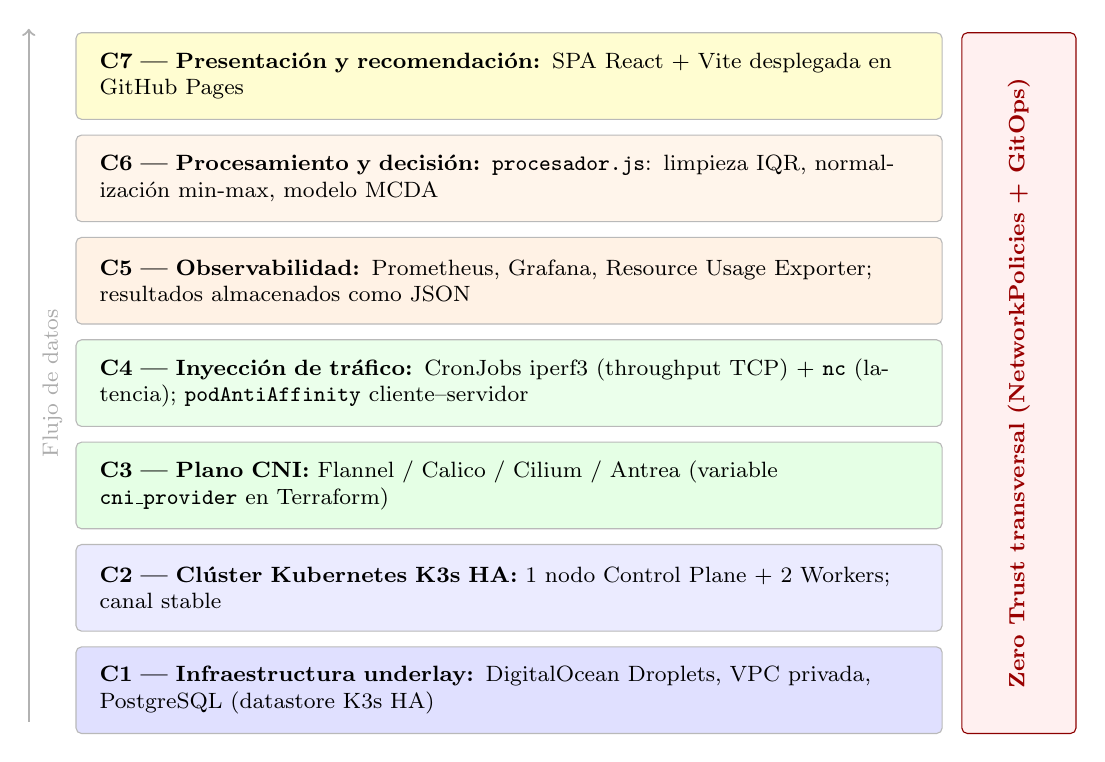
\begin{tikzpicture}[font=\footnotesize]
\tikzset{lay/.style={draw=gray!55, minimum width=11cm, minimum height=1.1cm,
    text width=10.4cm, align=left, inner sep=4pt, rounded corners=2pt}}

\node[lay, fill=blue!12] at (0,0.0)
    {\textbf{C1 --- Infraestructura underlay:} DigitalOcean Droplets, VPC privada, PostgreSQL (datastore K3s HA)};
% VERIFICAR: anclar versión exacta de K3s también aquí cuando se recupere de los logs
\node[lay, fill=blue!8] at (0,1.3)
    {\textbf{C2 --- Clúster Kubernetes K3s HA:} 1 nodo Control Plane + 2 Workers; canal stable};
\node[lay, fill=green!10] at (0,2.6)
    {\textbf{C3 --- Plano CNI:} Flannel / Calico / Cilium / Antrea (variable \texttt{cni\_provider} en Terraform)};
\node[lay, fill=green!8] at (0,3.9)
    {\textbf{C4 --- Inyección de tráfico:} CronJobs iperf3 (throughput TCP) + \texttt{nc} (latencia); \texttt{podAntiAffinity} cliente--servidor};
\node[lay, fill=orange!10] at (0,5.2)
    {\textbf{C5 --- Observabilidad:} Prometheus, Grafana, Resource Usage Exporter; resultados almacenados como JSON};
\node[lay, fill=orange!8] at (0,6.5)
    {\textbf{C6 --- Procesamiento y decisión:} \texttt{procesador.js}: limpieza IQR, normalización min-max, modelo MCDA};
\node[lay, fill=yellow!18] at (0,7.8)
    {\textbf{C7 --- Presentación y recomendación:} SPA React + Vite desplegada en GitHub Pages};

% Zero Trust transversal bar
\fill[red!6, draw=red!55!black, rounded corners=2pt] (5.75,-0.55) rectangle (7.20,8.35);
\node[rotate=90, font=\footnotesize\bfseries, text=red!60!black] at (6.475,3.90)
    {Zero Trust transversal (NetworkPolicies + GitOps)};

% Data flow arrow
\draw[->, thick, gray!60] (-6.10,-0.40) -- (-6.10,8.40);
\node[rotate=90, font=\footnotesize, text=gray!65] at (-5.80,3.90) {Flujo de datos};

\end{tikzpicture}
\caption{Arquitectura por capas del testbed experimental.}
\label{fig:arquitectura-capas}
\end{figure}
\shorthandon{>}

\section{Trazabilidad y Requisitos de Diseño}

El diseño no se planteó como una arquitectura aislada, sino como respuesta directa al problema formulado en el anteproyecto: las organizaciones adoptan Kubernetes como plataforma de orquestación, pero la calidad final del despliegue depende del plano de red, de la selección del CNI y del control de las comunicaciones internas del clúster \cite{ref29}. La Tabla~\ref{tab:trazabilidad-diseno} hace explícita la correspondencia entre cada necesidad, su objetivo asociado y la decisión de diseño que la atiende.

\begin{table}[htbp]
\centering
\scriptsize
\caption{Trazabilidad entre problema de investigación, objetivo y decisión de diseño.}
\label{tab:trazabilidad-diseno}
\begin{tabularx}{\textwidth}{|Y|Y|Y|}
\hline
\textbf{Necesidad identificada} & \textbf{Objetivo asociado} & \textbf{Respuesta de diseño} \\
\hline
Comparar CNIs sin depender de recomendaciones informales. & Evaluar cuantitativamente Calico, Cilium, Flannel y Antrea en escenarios controlados. & Testbed reproducible sobre Kubernetes, ejecución automatizada y consolidación de métricas por CNI. \\
\hline
Controlar el riesgo de comunicaciones internas abiertas. & Evaluar políticas de red seguras y automatizadas. & NetworkPolicies bajo enfoque Zero Trust, casos de denegación por defecto y segmentación por capas. \\
\hline
Convertir resultados técnicos heterogéneos en una decisión comprensible. & Definir criterios, umbrales y ponderaciones para comparación objetiva. & Modelo MCDA con criterios de rendimiento, eficiencia de recursos e impacto de seguridad. \\
\hline
Apoyar a una organización que necesita seleccionar y configurar un CNI. & Implementar un prototipo funcional de recomendación. & Prototipo web que consume datos procesados, aplica perfiles de decisión y explica la recomendación. \\
\hline
Evitar sobredimensionamiento de infraestructura. & Relacionar desempeño de red con consumo de CPU y memoria. & Captura de recursos del CNI mediante Prometheus y cálculo de eficiencia relativa por perfil. \\
\hline
\end{tabularx}
\end{table}

De este planteamiento se derivan cinco requisitos de diseño. La \textbf{reproducibilidad} se obtiene mediante infraestructura como código, despliegue declarativo y automatización de experimentos. El \textbf{aislamiento de variables} mantiene constante todo elemento distinto del CNI ---proveedor, tipo de instancia, versión de Kubernetes, topología y duración---. La \textbf{medición integral} evalúa el CNI por rendimiento de red, eficiencia de recursos e impacto de seguridad, y no solo por throughput. La \textbf{trazabilidad de la evidencia} exige que cada dato conserve su origen. La \textbf{compatibilidad con la operación real} se logra empleando objetos y patrones nativos de Kubernetes ---Deployments, CronJobs, ArgoCD--- cercanos a la práctica de los equipos de operaciones.

\section{Prototipo Recomendador}

El prototipo recomendador es la capa de interacción entre el modelo matemático y el usuario final. Su salida comprende tres niveles: la recomendación directa (qué CNI se sugiere), la justificación (qué métricas la explican) y la orientación de configuración (qué consideraciones debe atender el usuario al desplegar ese CNI), estructura que responde al objetivo específico 4 del anteproyecto \cite{ref29}. Se implementó como SPA con React~19, Vite~7 y Tailwind CSS~3; el \emph{build} de producción se despliega en GitHub Pages, y la actualización de datos encadena \texttt{procesador.js} ---que genera \texttt{cni-data.json}--- con la inyección de esos datos en el \emph{bundle}.

\section{Alcance y Límites del Diseño}

El diseño se limita a evaluar CNIs en un testbed controlado sobre Kubernetes y no pretende generalizar automáticamente los resultados a cualquier proveedor, versión o hardware. Emplea tráfico TCP controlado como señal principal y no asume que una mayor complejidad implique un mejor resultado. La solución se concibió para sostener una mejora continua: a medida que se incorporen nuevas corridas o versiones de CNIs, el pipeline puede recalcular los puntajes. En lugar de entregar una decisión congelada, ofrece un método para decidir con evidencia actualizable: técnicamente, reemplaza opiniones por datos medidos en condiciones reproducibles; económicamente, conocer el consumo de CPU de cada CNI por unidad de tráfico permite dimensionar la infraestructura sin márgenes precautorios excesivos \cite{ref29}.

